%% storify: close-out of the counterfactual covariate testbed (PI request 2026-10-30).
%% Anchor: the question "Do the recorded experimental covariates carry enough information
%% to map one measurement of a track onto another measurement of the same material?" and
%% everything under it. Edit THIS file. Run `python3 build_story.py` to write story.tex,
%% then `latexmk -pdf story.tex`. Never edit story.tex by hand: the build overwrites it.
%%
%% numbers   every measured number is a macro the build defines in the data slot below,
%%           read from results/{t130,t136,t137,t138,t139,t142,h15,h19,t122,t125}.
%% typed     design constants only, each in \lit{}: 7 tracks, 10 settings, 130 products,
%%           30M and 50M base depths, 15M/7.5M/3.75M depth arms, 36 and 50 bp read
%%           lengths, antibody proxy 50% and 90%, 25 bp bins, 1 kb bins, chr19 + chr21,
%%           3 seeds, the PI's bar 0.5 and 2 x seed range, the swap bar 0.1, log10 and
%%           log2, k = 4-5 count units per read, ratios 2 and 4, 2 test chromosomes,
%%           mapping filter 0.
%%
%% REFRESH after any re-run of the t136 readings: copy results/t136/{checks_readings,
%% m1_heldout_table}.tsv, rebuild, and re-read the paragraph "Arm-to-arm training" and the
%% depth-law row of the goals table. The grid is complete (42 of 42 runs, 2026-10-31).
\documentclass[pdflatex,sn-mathphys-num,iicol]{sn-jnl}

% crux-sources: __SOURCES__

\usepackage{graphicx}
\usepackage{amsmath}
\usepackage{booktabs}
\usepackage{array}
\usepackage{xcolor}
\usepackage{tikz}
\usetikzlibrary{positioning,arrows.meta,calc}
\usepackage{pgfplots}
\pgfplotsset{compat=1.18}
\usepackage{pgfplotstable}

% A design constant typed in prose, e.g. \lit{95}. It renders its argument unchanged.
\newcommand{\lit}[1]{#1}

% One colour per design and per mark class; defined once, reused everywhere.
\definecolor{dA}{HTML}{9A9A9A}
\definecolor{dB}{HTML}{3F7D7A}
\definecolor{dC}{HTML}{B5462E}
\definecolor{dD}{HTML}{4B5FA6}
\definecolor{cDn}{HTML}{B5462E}
\definecolor{cNar}{HTML}{3F7D7A}
\definecolor{cBr}{HTML}{4B5FA6}

% __DATA__

\raggedbottom

\begin{document}

\title[Counterfactual covariate testbed]{Recorded processing covariates map a track onto its counterfactual on trained pairs, but the map does not carry to unseen pairs}

\author{\fnm{Mehdi} \sur{Foroozandeh}}
\affil{\orgname{CANDI project, private close-out draft, \today}}

\abstract{We asked whether recorded processing covariates carry enough information to map one
measurement of an epigenomic track onto another of the same material. We built counterfactual arms of \lit{7} tracks, each changing one of \lit{10} processing
settings, and trained a generator that reads the covariates and outputs the map. On trained
depth pairs, the better designs close \gcBDLo{} to \gcBDHi{} of the gap from a covariate-free
monotone map to the exact oracle (seed range at most \gcBDnoiseHi{} of that gap). On unseen
pairs the gain over a scrambled-covariate twin falls from \relCntTr{} to \relCntSame{}, and
no design meets the depth law. All readings are exploratory, not judged.}

\keywords{epigenomics, experimental covariates, counterfactual data, sequencing depth}

\maketitle

\section{Motivation and background}\label{sec:motivation}

CANDI imputes epigenomic tracks from raw counts and reads experimental covariates (depth,
run type, read length) on both sides; its zero-shot claims rest on that conditioning. Inside
CANDI it cannot be tested alone: training tracks differ in biology and covariates at once, and
the covariates are collinear (they change together). Depth has a closed form, binomial
thinning; the other settings have none. Missing was data where one setting's true effect is known. Our question: do the recorded covariates carry enough information to map one
measurement of a track onto another of the same material?

\section{Methods}\label{sec:methods}

\paragraph{Counterfactual arms.} We took \lit{7} ENCODE imputation-challenge tracks (one
DNase-seq, three narrow and three broad histone marks), each processed to a base of \lit{30}M
reads (DNase \lit{50}M) and to arms that change one setting: depth (\lit{15}M,
\lit{7.5}M, \lit{3.75}M subsamples of the base), read length (\lit{36}, \lit{50}~bp), mapping
filter, duplicate removal, paired-end, an antibody proxy (\lit{50}\% or \lit{90}\% control
reads), fragment extension and three control settings: \lit{130} products. Each product was
split into two pseudoreplicate halves (random halves of its reads).

\paragraph{Model and competitors.} A generator $g$ reads the source and target covariates $C$,
$C'$ and outputs a map $f$; $f(X)$ predicts the target as negative binomial (NB) counts per
\lit{25}~bp bin, or as $-\log_{\lit{10}} p$ (Fig.~\ref{fig:design}). Four designs of $f$ rise
in capacity: per-bin affine (A), per-bin monotone curve (B), kernel plus curve (C) and a
conditioned convolutional network (D). The competitors are the no-covariates twin (covariates
scrambled), one-warp (a covariate-free monotone map per pair) and an oracle. The score is the
NB CRPS (continuous ranked probability score, distance from forecast to observation), split
into a shape part and a scale error. Gap closed is
$(D_\text{one-warp}-D_\text{model})/(D_\text{one-warp}-D_\text{oracle})$. The bar, set before
reading, is gap closed $\ge \lit{0.5}$ in every mark class and a gain above \lit{2}$\times$ the
seed range (largest minus smallest of \lit{3} seeds). Scoring uses held-out \lit{chr19} and
\lit{chr21}.

\paragraph{Floor and maps.} The resampling floor thins the halves along a depth ladder and
reads \lit{1}~kb shape (one minus Spearman) and peak height. Regional maps fit
signal level as the null, then read GC, mappability, repeats and peak context, beside a
shuffle control.

\paragraph{Two corrections.} First, the floor was planned as the depth oracle. But a depth arm
shares its base's reads, so the floor sat above one-warp and inverted the interval. The oracle
is now the exact nested-read oracle: binomial thinning of the base count, and its Bayes
posterior in reverse. The real arms have \dispLo{} to \dispHi{} of the binomial
variance. Second, a read adds one count to each \lit{25}~bp bin it covers ($k=\lit{4}$--\lit{5}); the
first floor thinned single counts, so multi-bin sums were about $\sqrt{k}$ too smooth. We
rebuilt it by thinning whole reads.

\begin{figure}[t]
\centering
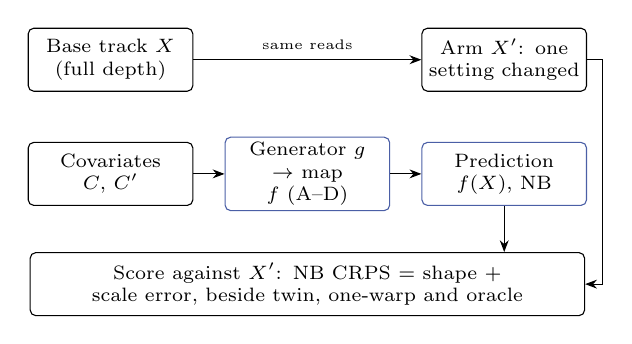
\begin{tikzpicture}[box/.style={draw, rounded corners=2pt, align=center, font=\scriptsize,
    minimum height=0.8cm, text width=1.95cm, inner sep=2pt}, >={Stealth[length=1.5mm]}]
  \node[box] (base) at (0,0) {Base track $X$\\ (full depth)};
  \node[box] (arm) at (5.0,0) {Arm $X'$: one\\ setting changed};
  \node[box] (cov) at (0,-1.45) {Covariates\\ $C$, $C'$};
  \node[box, draw=dD] (g) at (2.5,-1.45) {Generator $g$\\ $\to$ map $f$ (A--D)};
  \node[box, draw=dD] (pred) at (5.0,-1.45) {Prediction\\ $f(X)$, NB};
  \node[box, text width=6.9cm] (score) at (2.5,-2.85) {Score against $X'$: NB CRPS = shape +
    scale error, beside twin, one-warp and oracle};
  \draw[->] (base) -- node[above, font=\tiny] {same reads} (arm);
  \draw[->] (cov) -- (g);
  \draw[->] (g) -- (pred);
  \draw[->] (pred) -- (pred |- score.north);
  \draw[->] (arm.east) -- ++(0.2,0) |- (score.east);
\end{tikzpicture}
\caption{Design. Each arm reprocesses the base's reads with one setting changed. The generator
reads both covariate sets and outputs the map that turns the base into a predicted arm, scored
beside three competitors.}\label{fig:design}
\end{figure}

\section{Results and discussion}\label{sec:results}

\paragraph{Depth: the covariates close most of the gap.} From base to arm, designs B to D close
\gcBDLo{} to \gcBDHi{} of the gap in every mark class (Fig.~\ref{fig:results}a), with a seed
range of \gcBDnoiseLo{} to \gcBDnoiseHi{} in gap units; the gain beats \lit{2}$\times$ the seed
range in \nBDgain{} of \nBDcells{} cells. In narrow marks, design B scores \wModel{}
(\wModelOS{} shape + \wModelSE{} scale error), one-warp \wWarp{} (\wWarpOS{} + \wWarpSE{}) and
the oracle \wOra{} (\wOraOS{} + \wOraSE{}), against \lit{2}$\times$ seed range \wSeed{}. The
interval is small (\ivBLo{} to \ivBHi{}). Design A shows no gain in DNase and narrow marks (\gcALo{} to \gcAHi{}, seed range \gcAnoiseLo{} to
\gcAnoiseHi{}). From arm to base, C and D pass the per-bin oracle (\gcCDabLo{} to \gcCDabHi{}) by
reading neighbouring bins.

\paragraph{Run type: better than one-warp, no valid ceiling.} Paired-end reprocessing is not a
subsample, so the floor stays its oracle. In narrow marks the floor, \peFloor{} (\peFloorOS{} +
\peFloorSE{}), lies above one-warp, \peWarp{} (\peWarpOS{} + \peWarpSE{}), so gap closed cannot
be read. The model beats one-warp by \peGainLo{} to \peGainHi{} in \nPeHistSig{} of \nPeHist{}
histone cells, each above \lit{2}$\times$ the seed range (\peSeedLo{} to \peSeedHi{}); in DNase,
\nPeDnSig{} of \nPeDn{} cells.

\paragraph{Unseen pairs.} The relative count gain over the twin falls from \relCntTr{} on
trained pairs to \relCntSame{} on unseen pairs of one setting (\relCntCross{} for two); in $p$,
from \relPTr{} to \relPSame{} (\relPCross{}). It clears \lit{2}$\times$ the seed range in
\nMetTr{} of \nCfg{} configurations trained and \nMetSame{} of \nCfg{} unseen. Only the control settings keep their $p$ gain (\ctlPTrLo{} to \ctlPTrHi{}
trained, \ctlPSameLo{} to \ctlPSameHi{} unseen; seed range at most \ctlWobHi{}). Told $C'=C$,
no design returns its input (\swapLo{} to \swapHi{}, bar \lit{0.1}).

\paragraph{The depth law.} The real arms obey it within \lawData\% (\nLawPairs{} pairs). On
unseen arm-to-arm pairs the direct map misses it (median $|\log_{\lit{2}}|$ scale error
\lawRef{}, seed range \lawRefS{}); two trained maps chained through the base come closer
(\lawVia{}, seed range \lawViaS{}).

\paragraph{Arm-to-arm training (complete).} One added arm-to-arm pair
per track (ratio \lit{4}) brings the held-out ratio-\lit{2} error to \lawArm{} (seed range
\lawArmS{}), closing \cOneGap{} of the gap to the chained map (bar \lit{0.5}); it passes the
transfer bar (\cThreeHeld{} against \cThreeBar{}) and keeps the base fit (\fitArm{} against
\fitRef{}). But the predicted distribution gets worse: CRPS \crArm{} (\crArmOS{} + \crArmSE{}, seed range \crArmS{}) against \crRef{}
(\crRefOS{} + \crRefSE{}) direct and \crVia{} (\crViaOS{} + \crViaSE{}) chained, a gap closed
of \cFourGap{}, mostly scale error in DNase. Both arms are complete and
both controls pass, so the reading is final: \ruleReading{} (not judged). The
every-pair second arm (not checked) reaches the chained map: CRPS \crArmTwo{} (\crArmTwoOS{} + \crArmTwoSE{}, seed
range \crArmTwoS{}), gap closed \crArmTwoGap{}.

\paragraph{The floor, and where settings act.} Whole-read thinning reproduces the real depth
halves (\lit{1}~kb shape ratio \realRead{}, against \realUnit{} for count thinning). At
\lit{3.75}M reads per half the narrow shape floor is \shLowNar{}, not \shLowUnitNar{}
(Fig.~\ref{fig:results}b; seed range at most \shSpreadHi{}). Signal level explains
\lvlFifteenLo{} to \lvlFifteenHi{} of the per-bin disagreement; regional features add at most
\featMax{} (shuffle \shufMax{}). Depth acts uniformly: its residual equals its whole-read null
(DNase \depArm{} against \depNull{}). The mapping filter does not: feature gain \mapqZeroLo{} to
\mapqZeroHi{} (Fig.~\ref{fig:results}c), against at most \floorFeatHi{} for the floor.

\begin{figure*}[t]
\centering
\begin{tikzpicture}
\begin{axis}[name=pa, width=0.33\textwidth, height=4.6cm,
    title={\small (a) Gap closed, depth, base to arm},
    ymin=-2.2, ymax=2.2, xmin=-0.5, xmax=2.5,
    xtick={0,1,2}, xticklabels={DNase, narrow, broad}, xtick style={draw=none},
    xticklabel style={text height=1.5ex, text depth=0.3ex},
    ylabel={Gap closed}, tick label style={font=\scriptsize}, label style={font=\footnotesize},
    extra y ticks={0,0.5}, extra y tick labels={},
    extra y tick style={grid=major, grid style={gray!60, thin}},
    legend style={font=\tiny, at={(0.5,0.98)}, anchor=north, draw=none, fill=none},
    legend columns=4]
  \addplot[only marks, mark=*, mark size=1.4pt, color=dA, error bars/.cd, y dir=both, y explicit]
    table[x=x, y=gc, y error=err]{\tblGapA};
  \addlegendentry{A}
  \addplot[only marks, mark=*, mark size=1.4pt, color=dB, error bars/.cd, y dir=both, y explicit]
    table[x=x, y=gc, y error=err]{\tblGapB};
  \addlegendentry{B}
  \addplot[only marks, mark=*, mark size=1.4pt, color=dC, error bars/.cd, y dir=both, y explicit]
    table[x=x, y=gc, y error=err]{\tblGapC};
  \addlegendentry{C}
  \addplot[only marks, mark=*, mark size=1.4pt, color=dD, error bars/.cd, y dir=both, y explicit]
    table[x=x, y=gc, y error=err]{\tblGapD};
  \addlegendentry{D}
\end{axis}
\begin{axis}[name=pb, at={(pa.east)}, anchor=west, xshift=1.2cm, width=0.33\textwidth, height=4.6cm,
    title={\small (b) Shape floor against depth},
    xlabel={Reads per half (M)}, ylabel={$1-\rho$, 1 kb bins},
    xtick={0.907,1.907,2.907,3.907,4.907}, xticklabels={1.9,3.75,7.5,15,30},
    ymin=0, ymax=1.6, tick label style={font=\scriptsize}, label style={font=\footnotesize},
    legend style={font=\tiny, at={(0.98,0.98)}, anchor=north east, draw=none, fill=none},
    legend columns=1]
  \addplot[color=cNar, mark=*, mark size=0.9pt] table[x=x, y=y]{\tblShReadNar};
  \addlegendentry{narrow}
  \addplot[color=cBr, mark=*, mark size=0.9pt] table[x=x, y=y]{\tblShReadBr};
  \addlegendentry{broad}
  \addplot[color=cDn, mark=*, mark size=0.9pt] table[x=x, y=y]{\tblShReadDn};
  \addlegendentry{DNase}
  \addplot[color=cNar, dashed, mark=o, mark size=0.9pt, forget plot] table[x=x, y=y]{\tblShUnitNar};
  \addplot[color=cBr, dashed, mark=o, mark size=0.9pt, forget plot] table[x=x, y=y]{\tblShUnitBr};
  \addplot[color=cDn, dashed, mark=o, mark size=0.9pt, forget plot] table[x=x, y=y]{\tblShUnitDn};
\end{axis}
\begin{axis}[at={(pb.east)}, anchor=west, xshift=1.3cm, width=0.36\textwidth, height=4.6cm,
    ybar, bar width=3pt,
    title={\small (c) Regional feature gain per setting},
    ymode=log, log origin=infty, ymin=1e-5, ymax=0.5, ylabel={Extra $R^{\lit{2}}$},
    xtick=data, xticklabels from table={\tblKnob}{lab}, xtick style={draw=none},
    xticklabel style={rotate=40, anchor=north east, font=\tiny},
    enlarge x limits=0.08, tick label style={font=\scriptsize}, label style={font=\footnotesize},
    extra y ticks={3e-5}, extra y tick labels={},
    extra y tick style={grid=major, grid style={gray, dashed}},
    legend style={font=\tiny, at={(0.03,0.97)}, anchor=north west, draw=none, fill=none},
    area legend]
  \addplot[fill=cNar, draw=none] table[x=x, y=nar]{\tblKnob};
  \addlegendentry{narrow}
  \addplot[fill=cBr, draw=none] table[x=x, y=br]{\tblKnob};
  \addlegendentry{broad}
\end{axis}
\end{tikzpicture}
\caption{(a) Gap closed from one-warp to the nested-read oracle on depth pairs, base to arm,
one generator per track. Error bars are \lit{2}$\times$ the seed range in gap units; grid lines
mark zero and the \lit{0.5} bar. (b) The \lit{1}~kb shape floor (median over products) along
the thinning ladder; the rightmost point is extrapolated. Solid lines thin whole reads, dashed
lines thin single counts; the seed range is at most \shSpreadHi{}, smaller than the marks.
(c) Extra $R^{\lit{2}}$ that GC, mappability, repeats and peak context add to the signal-level null on
the one-warp residual (median over tracks); the dashed line is the largest shuffle control.}
\label{fig:results}
\end{figure*}

\begin{table*}[t]
\caption{Each original goal, its status and one line of evidence. Status is a proposal for the
PI to sign. Met: the question has a full reading. Partly met: part of it is read. Answered: the
aim was not met, but the reading answers the question well enough to act.}
\label{tab:goals}
\footnotesize
\begin{tabular}{@{}>{\raggedright\arraybackslash}p{0.26\textwidth}>{\raggedright\arraybackslash}p{0.1\textwidth}>{\raggedright\arraybackslash}p{0.59\textwidth}@{}}
\toprule
Goal & Status & Evidence (not judged) \\
\midrule
Do covariates map one measurement onto another? (main question) & Partly met & Beat the scrambled twin on trained pairs; count gain \relCntTr{} falls to \relCntSame{} unseen; swap and depth-law checks unmet \\
Depth conditioning beyond one-warp & Met & Designs B--D close \gcBDLo{}--\gcBDHi{} of the gap; gain above \lit{2}$\times$ seed range in \nBDgain{}/\nBDcells{} cells; design A no gain \\
Run-type conditioning beyond one-warp & Partly met & Beats one-warp in \nPeHistSig{}/\nPeHist{} histone cells by \peGainLo{}--\peGainHi{}; no valid ceiling; DNase \nPeDnSig{}/\nPeDn{} \\
Read-selection settings & Partly met & Count gain over twin \readTrLo{}--\readTrHi{} trained (seed range \readWobLo{}--\readWobHi{}); $p$ gain \readPSameLo{}--\readPSameHi{} unseen; one-warp bar not scored \\
Control and caller settings & Partly met & $p$ gain \ctlPTrLo{}--\ctlPTrHi{} trained, \ctlPSameLo{}--\ctlPSameHi{} unseen (seed range $\le$ \ctlWobHi{}); oracle interval negative, so bar unreadable \\
Capacity of the map & Answered & A monotone curve suffices in counts; more capacity does not fix unseen pairs; $p$ explodes in B--D \\
Depth offset & Answered & Helps design A only: DNase CRPS \oldA{} (\oldAOS{} + \oldASE{}) to \offA{} (\offAOS{} + \offASE{}), gain \offGain{} against bar \offBar{}; other designs \offBDclear{}/\offBDn{}; depth law met in \offLawIn{}/\offLawN{} cells \\
Counts-to-$p$ map & Answered & Caller's formula plus learned correction, log CRPS \hBest{} $\pm$ \hBestW{} (\hBestOS{} + \hBestSE{}), against \hAff{} (\hAffOS{} + \hAffSE{}) for an affine map; one track \\
Why the depth law is missed & Partly met & Not the pseudocount, loss or model size; arm-to-arm training meets the law (gap closed \cOneGap{}) but CRPS fails (\cFourGap{}); grid complete, controls pass; every-pair arm closes \crArmTwoGap{} (not checked) \\
Does CANDI's training let it correct other covariates? & Partly met & Told read length or run type, CANDI moves its level; per-region tracking unreadable (floor failed its depth control); probe parked \\
Which settings move a track most & Met & On one shared peak set: peak height above floor \nPhAbove{}/\nPh{} (\phRatioLo{}--\phRatioHi{}$\times$), shape \nShAbove{}/\nSh{} \\
How much resampling alone moves a track & Met & \lit{1}~kb shape floor at \lit{30}M: narrow \shThirtyNar{}, broad \shThirtyBr{}, DNase \shThirtyDn{} (seed range $\le$ \shSpreadHi{}); level, not region, sets it \\
Where along the genome settings act & Met & Depth uniform (residual = null); mapping filter \mapqZeroLo{}--\mapqZeroHi{}, read length \cropFeatLo{}--\cropFeatHi{} extra $R^{\lit{2}}$, in low-mappability bins \\
\botrule
\end{tabular}
\end{table*}

\section{Conclusion}\label{sec:conclusion}

On trained pairs the covariates carry the information: for depth they close most of the gap
to the oracle; for run type and control settings they beat a covariate-free map. On
unseen pairs the gain shrinks and the direct map misses the depth law. Two arm-to-arm
pairs fix the law but not the distribution; every pair fixes both (not checked). Table~\ref{tab:goals} gives each goal's status. Limitations: \lit{7} tracks, \lit{3} seeds, \lit{2} test chromosomes, and no ceiling for the
run-type and control claims.

\paragraph{What carries to CANDI.} Use the full-depth track as the depth base, with depth as a
fixed offset and no positional term. An NB-like, level-dependent spread describes the
resampling floor. Read length and mapping filters act in low-mappability regions, so their
correction needs sequence or mappability input. Conditioning will not carry to setting
combinations that training never paired.

Next steps, without ranking:
\begin{itemize}
\item \textbf{A full-depth oracle for run type and control settings.} Moderate; gives those
claims a ceiling.
\item \textbf{Augment CANDI with counterfactual pairs.} Costly; tests whether the trained-pair
gain carries into CANDI.
\end{itemize}

\end{document}
